%!TEX root = ../dokumentation.tex

\chapter{Couchbase DB (Document)} \label{ch:couchbase}
\chapterauthor{Taha Erkoc, Lara Hennes, Christian Herzgen and Ilya Suplin}

Migrating relational databases to \ac{NoSQL} databases is a problem many companies need to face when they adapt to new standards in the industry. Doing so can be a tedious process as there are many different \ac{NoSQL} databases with their own query language to choose from and developers need their time to adapt.\newline This is where Couchbase DB comes into play. It is a document-oriented database and saves data in \ac{JSON} documents, which makes it a semi-structured database. With its multi-model trait and unique query language \ac{N1QL} Couchbase DB is the fastest document oriented database to adapt to. This is mainly because \ac{N1QL} features the same syntax as \ac{SQL}. \parencite{BigdataInsiderOnCouchbase}

\section{History}
Couchbase was formed as a fusion between CouchOne and Membase in 2011, two companies with very different approaches to databases. CouchOne with its still known database Couch DB focussed on mobile and offline use cases to support unreliable network connections. Opposed to that Membase worked on scaling important apps and performance, by using the technical development of servers, as the system behind Zynga, a large browser game company. Couchbase was born and with it the Couchbase Server System, where Couchbase DB is running. Together they created a database, that is scalable both up and down aswell as supporting offline use cases.  \parencite{CouchOne-Membase-Fusion}\newline
Back then it was a key-value database, but with the release of Couchbase Server 2.0 in 2012 it was transformed to the now known document-oriented database. Throughout the years Couchbase improved their product and in 2021 they released Couchbase Server 7.0, which is the current major version we will talk about. \parencite{CouchbaseAbout}

\section{Architecture}
Knowledge of a databases architecture is one of the key factors to understanding its use. Couchbase offers an easy to use and implement architecture, that even beginners will understand.
\begin{figure}[H]
    \centering
        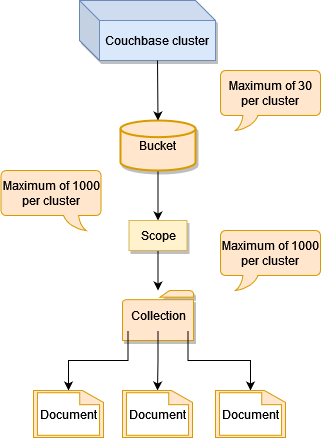
\includegraphics[scale=0.8]{images/CouchbaseArchitecture.drawio.png}
    \caption{Couchbase Architecture \parencite{CouchbaseArchitecture}}
    \label{fig:CouchbaseArchitecture}
\end{figure}
This overview of a Couchbase cluster is everything one needs to get started. The \ac{JSON} documents are stored in collections, which are put into scopes. These scope are further put into buckets, that are the top layer of storage. \parencite{CouchbaseIntroduction}\newline
With this one can get a personal database running, but how is it possible to scale a database to enterprise levels? A cluster consists of one or multiple interchangeable nodes, that communicate peer-to-peer and can stand alone. One node can be any computer system running the Couchbase Server system. \parencite{CouchbasePaper}\newline Each node has a Cluster Manager, which is responsible for node coordination and also acts as an interface for users to administrate the cluster. Starting out with the first node, there will be four services running:
\begin{itemize}
    \item Data Service
    \item Index Service
    \item Query Service
    \item Search Service
\end{itemize}
These services can be configured across nodes, so that a cluster can consist of four nodes with each running one of the services. Running the same service on multiple nodes is also possible. \parencite{CouchbaseIntroduction} \newline
To sum up, every node in a cluster has a cluster manager and storage as seen in (fig \ref{fig:CouchbaseArchitecture}) aswell as services, that can be spread across nodes. This allows Couchbase to implement \ac{MDS} to their database, that offers the opportunity for users not only to scale-up, but also scale-out their database. \parencite{CouchbasePaper}


\section{API}
The industry evolved to support more work from home or out of office, but users still want to administrate and work on their database. This is the reason why most \ac{NoSQL} databases support an \ac{API}, which makes administrating over \ac{HTTP} possible and easy to use.\newline
Couchbase DB provides an \ac{REST} \ac{API}, that supports various functions from cluster creation to managing nodes and retrieving statistics of a database. Currently there are thirteen different \ac{REST} \acp{API} to use. The most important ones being Nodes and Clusters \ac{API}, Buckets \ac{API}, Scopes and Collections \ac{API} and Memory and Storage \ac{API}. With these users can create and manage their clusters and setup an entire database configuring different buckets, collections and storage allocation. If the database is setup and users want to start using it, the Query Service \ac{API}, which supports \ac{N1QL} queries, or the Search Service, which provides full text searches in the database, is what they need. \parencite{CouchbaseAPI}\newline
There is much more functionality to explore with the rest of the different \acp{API}. Definitely check them out before starting with the Couchbase DB cluster.


\section{Advantages \& Disadvantages}

\section{Improvement compared to relational database design}

\section{\ac{CAP}-Theorem}

\section{Fields of Application}

\section{Installation and setup of database}

\subsection{Windows}


\subsection{Docker}
If the user wants to have multiple nodes, or does not have a clean system, we recommend to install Couchbase in a Docker Container. Couchbase has an official Docker image, which can be found in the Docker Hub.

\begin{lstlisting}
docker run -d --name db -p 8091-8096:8091-8096 -p 11210-11211:11210-11211 couchbase
\end{lstlisting}


\section{Example}

\section{Recommendation \& Conclusion}